\documentclass[]{article}
\usepackage{lmodern}
\usepackage{amssymb,amsmath}
\usepackage{ifxetex,ifluatex}
\usepackage{fixltx2e} % provides \textsubscript
\ifnum 0\ifxetex 1\fi\ifluatex 1\fi=0 % if pdftex
  \usepackage[T1]{fontenc}
  \usepackage[utf8]{inputenc}
\else % if luatex or xelatex
  \ifxetex
    \usepackage{mathspec}
  \else
    \usepackage{fontspec}
  \fi
  \defaultfontfeatures{Ligatures=TeX,Scale=MatchLowercase}
\fi
% use upquote if available, for straight quotes in verbatim environments
\IfFileExists{upquote.sty}{\usepackage{upquote}}{}
% use microtype if available
\IfFileExists{microtype.sty}{%
\usepackage{microtype}
\UseMicrotypeSet[protrusion]{basicmath} % disable protrusion for tt fonts
}{}
\usepackage[margin=1in]{geometry}
\usepackage{hyperref}
\hypersetup{unicode=true,
            pdfborder={0 0 0},
            breaklinks=true}
\urlstyle{same}  % don't use monospace font for urls
\usepackage{color}
\usepackage{fancyvrb}
\newcommand{\VerbBar}{|}
\newcommand{\VERB}{\Verb[commandchars=\\\{\}]}
\DefineVerbatimEnvironment{Highlighting}{Verbatim}{commandchars=\\\{\}}
% Add ',fontsize=\small' for more characters per line
\usepackage{framed}
\definecolor{shadecolor}{RGB}{248,248,248}
\newenvironment{Shaded}{\begin{snugshade}}{\end{snugshade}}
\newcommand{\AlertTok}[1]{\textcolor[rgb]{0.94,0.16,0.16}{#1}}
\newcommand{\AnnotationTok}[1]{\textcolor[rgb]{0.56,0.35,0.01}{\textbf{\textit{#1}}}}
\newcommand{\AttributeTok}[1]{\textcolor[rgb]{0.77,0.63,0.00}{#1}}
\newcommand{\BaseNTok}[1]{\textcolor[rgb]{0.00,0.00,0.81}{#1}}
\newcommand{\BuiltInTok}[1]{#1}
\newcommand{\CharTok}[1]{\textcolor[rgb]{0.31,0.60,0.02}{#1}}
\newcommand{\CommentTok}[1]{\textcolor[rgb]{0.56,0.35,0.01}{\textit{#1}}}
\newcommand{\CommentVarTok}[1]{\textcolor[rgb]{0.56,0.35,0.01}{\textbf{\textit{#1}}}}
\newcommand{\ConstantTok}[1]{\textcolor[rgb]{0.00,0.00,0.00}{#1}}
\newcommand{\ControlFlowTok}[1]{\textcolor[rgb]{0.13,0.29,0.53}{\textbf{#1}}}
\newcommand{\DataTypeTok}[1]{\textcolor[rgb]{0.13,0.29,0.53}{#1}}
\newcommand{\DecValTok}[1]{\textcolor[rgb]{0.00,0.00,0.81}{#1}}
\newcommand{\DocumentationTok}[1]{\textcolor[rgb]{0.56,0.35,0.01}{\textbf{\textit{#1}}}}
\newcommand{\ErrorTok}[1]{\textcolor[rgb]{0.64,0.00,0.00}{\textbf{#1}}}
\newcommand{\ExtensionTok}[1]{#1}
\newcommand{\FloatTok}[1]{\textcolor[rgb]{0.00,0.00,0.81}{#1}}
\newcommand{\FunctionTok}[1]{\textcolor[rgb]{0.00,0.00,0.00}{#1}}
\newcommand{\ImportTok}[1]{#1}
\newcommand{\InformationTok}[1]{\textcolor[rgb]{0.56,0.35,0.01}{\textbf{\textit{#1}}}}
\newcommand{\KeywordTok}[1]{\textcolor[rgb]{0.13,0.29,0.53}{\textbf{#1}}}
\newcommand{\NormalTok}[1]{#1}
\newcommand{\OperatorTok}[1]{\textcolor[rgb]{0.81,0.36,0.00}{\textbf{#1}}}
\newcommand{\OtherTok}[1]{\textcolor[rgb]{0.56,0.35,0.01}{#1}}
\newcommand{\PreprocessorTok}[1]{\textcolor[rgb]{0.56,0.35,0.01}{\textit{#1}}}
\newcommand{\RegionMarkerTok}[1]{#1}
\newcommand{\SpecialCharTok}[1]{\textcolor[rgb]{0.00,0.00,0.00}{#1}}
\newcommand{\SpecialStringTok}[1]{\textcolor[rgb]{0.31,0.60,0.02}{#1}}
\newcommand{\StringTok}[1]{\textcolor[rgb]{0.31,0.60,0.02}{#1}}
\newcommand{\VariableTok}[1]{\textcolor[rgb]{0.00,0.00,0.00}{#1}}
\newcommand{\VerbatimStringTok}[1]{\textcolor[rgb]{0.31,0.60,0.02}{#1}}
\newcommand{\WarningTok}[1]{\textcolor[rgb]{0.56,0.35,0.01}{\textbf{\textit{#1}}}}
\usepackage{longtable,booktabs}
\usepackage{graphicx,grffile}
\makeatletter
\def\maxwidth{\ifdim\Gin@nat@width>\linewidth\linewidth\else\Gin@nat@width\fi}
\def\maxheight{\ifdim\Gin@nat@height>\textheight\textheight\else\Gin@nat@height\fi}
\makeatother
% Scale images if necessary, so that they will not overflow the page
% margins by default, and it is still possible to overwrite the defaults
% using explicit options in \includegraphics[width, height, ...]{}
\setkeys{Gin}{width=\maxwidth,height=\maxheight,keepaspectratio}
\IfFileExists{parskip.sty}{%
\usepackage{parskip}
}{% else
\setlength{\parindent}{0pt}
\setlength{\parskip}{6pt plus 2pt minus 1pt}
}
\setlength{\emergencystretch}{3em}  % prevent overfull lines
\providecommand{\tightlist}{%
  \setlength{\itemsep}{0pt}\setlength{\parskip}{0pt}}
\setcounter{secnumdepth}{5}
% Redefines (sub)paragraphs to behave more like sections
\ifx\paragraph\undefined\else
\let\oldparagraph\paragraph
\renewcommand{\paragraph}[1]{\oldparagraph{#1}\mbox{}}
\fi
\ifx\subparagraph\undefined\else
\let\oldsubparagraph\subparagraph
\renewcommand{\subparagraph}[1]{\oldsubparagraph{#1}\mbox{}}
\fi

%%% Use protect on footnotes to avoid problems with footnotes in titles
\let\rmarkdownfootnote\footnote%
\def\footnote{\protect\rmarkdownfootnote}

%%% Change title format to be more compact
\usepackage{titling}

% Create subtitle command for use in maketitle
\newcommand{\subtitle}[1]{
  \posttitle{
    \begin{center}\large#1\end{center}
    }
}

\setlength{\droptitle}{-2em}

  \title{}
    \pretitle{\vspace{\droptitle}}
  \posttitle{}
    \author{}
    \preauthor{}\postauthor{}
    \date{}
    \predate{}\postdate{}
  
\geometry{paper=a4paper, margin=2.2cm}
\usepackage[defaultlines=10,all]{nowidow}
\usepackage{float}

\usepackage{fancyhdr}
\pagestyle{fancy}
\lhead{\rightmark}
\rhead{Projet de transcription de musique}

\makeatletter
\renewcommand{\fps@figure}{H}
\makeatother

\AtBeginDocument{\let\maketitle\relax}

\DeclareUnicodeCharacter{266D}{\ensuremath{\flat}}

%%%%%%%%%%%%%%%% COVER

\makeatletter
\setlength{\parindent}{0cm}
\setlength{\parskip}{1ex plus 0.5ex minus 0.2ex}
\newcommand{\hsp}{\hspace{20pt}}
\newcommand{\HRule}{\rule{\linewidth}{0.5mm}}
\makeatother

\begin{document}

\begin{titlepage}
  \begin{sffamily}
  \begin{center}
	
\includegraphics[width=0.8\textwidth]{img/INSA_logo}\\[2cm]

    \textsc{\huge Département Génie Mathématique}\\[0.7cm]
    %\textsc{\Large }\\[1.5cm]

    % Title
    \HRule \\[0.4cm]
    {\huge \bfseries Projet de transcription de musique \\[0.4cm]}
    \HRule \\[1cm]
	\textsc{\huge Projet semestriel -- semestre 8}\\[0.7cm]

    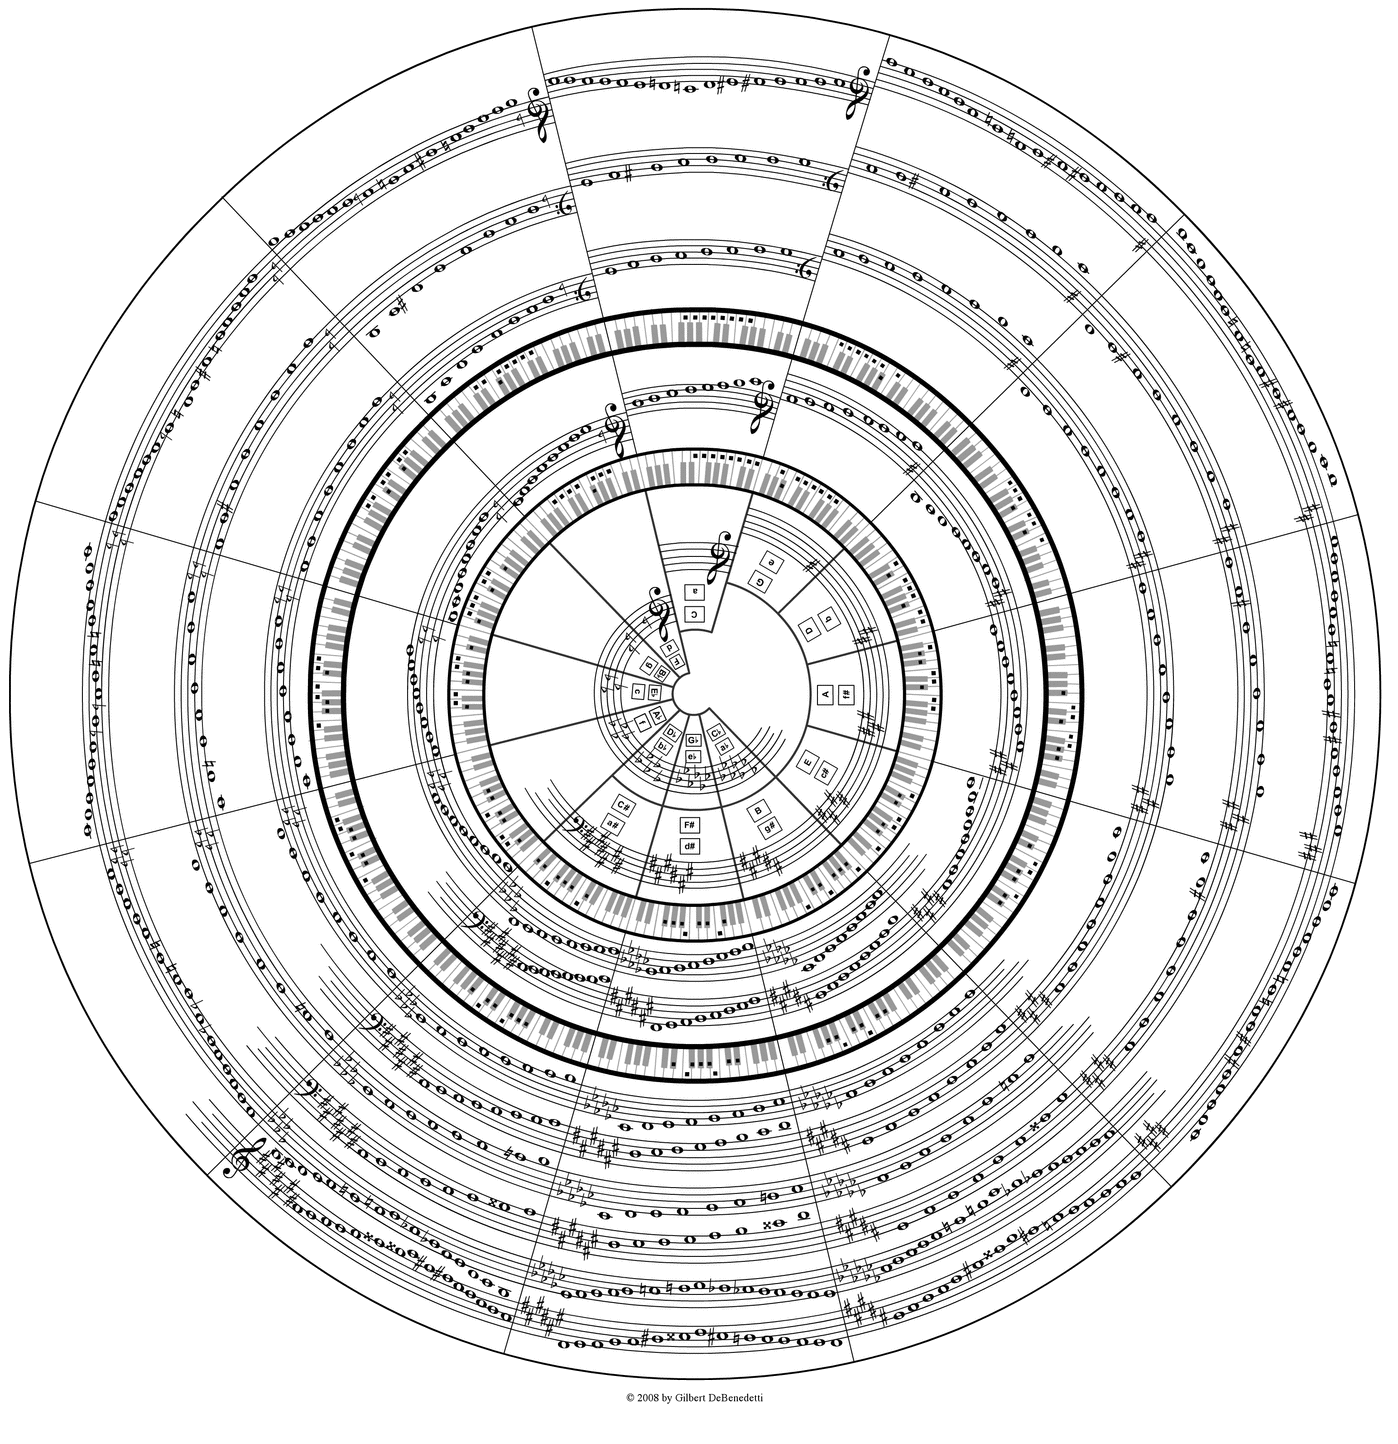
\includegraphics[width=.6\textwidth]{img/cover_img.png}~\\[1cm]

    % Author and supervisor
    \begin{minipage}{0.4\textwidth}
		\Large\raggedright
        Rand ASSWAD\\
		Ergi DIBRA\\
		Yuge SUN
    \end{minipage}
    \begin{minipage}{0.4\textwidth}
		\Large\raggedleft
		\emph{A l'attention de :}\\
		Mme. Natalie FORTIER
    \end{minipage}

	\vfill
    % Bottom of the page
    {\large 11 juin 2018}
  \end{center}
  \end{sffamily}
\end{titlepage}

{
\setcounter{tocdepth}{2}
\tableofcontents
}
\pagebreak

\begin{quote}
``La vie sans musique est tout simplement une erreur, une fatigue, un
exil.'' --- \textbf{Friedrich Nietzsche}
\end{quote}

\hypertarget{introduction}{%
\section{Introduction}\label{introduction}}

La musique peut être considérée comme la première langue parlée. Bien
que la musique soit un art, sa perception est un effort artistique aussi
bien que scientifique.

En effet, l'humain cherchait à caractériser la musique afin de pouvoir
la conserver et de la partager. Cette science a commencé par l'écriture
des chants hourrites sur des tablettes d'argile extraite d'Ougarit
(actuellement Latakié, Syrie) qui remontent approximativement à 1400 av.
J.-C. (Wikipédia 2018)

\begin{figure}
\centering
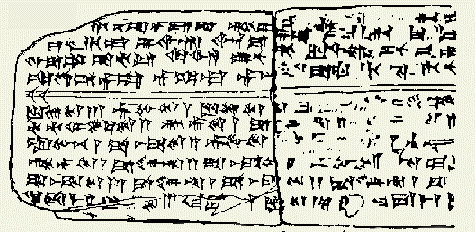
\includegraphics{img/Hurritische_hymne.png}
\caption{Dessin de la tablette de l'hymne à Nikkal (chant hourrite)}
\end{figure}

La notation musicale a évolué au cours de l'histoire, le système
occidental développé au moyen âge appelé ``\emph{solfège}'' est adopté
aujourd'hui par tous les musiciens du monde avec quelques variations. La
transcription d'une œuvre musicale est appelée une \emph{partition}.

Ce système de notation est fidèle à la perception humaine du son,
vis-à-vis la linéarité de fréquences et la reconnaissance du rythme. En
effet, on tappe les pieds suivant le rythme de la musique sans aucune
connaissance musicale, et la majorité de personnes est capable de
chanter une mélodie sans lire sa partition.

En revanche, un signal sonore contient les mêmes informations sous une
forme différente; l'espace de fréquences n'est pas linéaire et le rythme
n'est pas reconnaissable facilement.

Dans ce projet, nous avons étudié et implémenté des méthodes
d'interprétation de signaux sonores dans l'objectif de pouvoir produire
une partition de musique à partir d'un son enregistré.

Des nombreuses recherches ont été effectuées sur ce sujet et les
résultats obtenus sont certainement intéressants. Malheureusement, ces
méthodes ne traitent que des cas particuliers.

Nous nous sommes intéressés par ce domaine d'applications car il porte
un fort potentiel dans le futur. Ce projet nous a permis de faire notre
premier pas dans ce domaine et de mettre en place nos compétences en
mathématiques, en informatique et en musique.

\pagebreak

\hypertarget{signaux-sonores}{%
\section{Signaux sonores}\label{signaux-sonores}}

\hypertarget{musique-son}{%
\subsection{Musique \& Son}\label{musique-son}}

L'humain fait le lien entre la musique et le son dans son cerveau
instantanément sans le moindre d'efforts. Néanmoins, nous voudrions
établir ce lien de façon scientifique.

Un son possède des les caractéristiques suivants:

\begin{itemize}
\tightlist
\item
  Hauteur tonale (fréquence)
\item
  Durée
\item
  Intensité (énergie)
\item
  Timbre (source sonore)
\end{itemize}

La musique se caractérise par:

\begin{itemize}
\tightlist
\item
  \textbf{La mélodie:} la suite de phrases ou motifs sonores monophones
\item
  \textbf{L'harmonie:} l'ensemble de son différents simultanés
\item
  \textbf{Le rythme:} la suite de durées du son
\item
  \textbf{La nuance:} l'intensité relative du son
\item
  \textbf{Le timbre:} la nature du son / son source / son empreinte
\end{itemize}

Nous allons expliquer dans ce projet les notions de base de ce lien.

\hypertarget{son-harmonique}{%
\subsection{Son harmonique}\label{son-harmonique}}

Le son d'un résonateur acoustique comme une chorde ou une colonne d'air
est une onde stationnaire. On dit que tel son évoque un \textbf{pitch
défini}. Dans le cas des instruments de percussion, le son présente une
\emph{inharmonicité}. On dit que tel son évoque un \textbf{pitch
indéfini}. Dans ce projet on ne s'intéressera qu'au sons harmoniques de
pitch défini.

\begin{figure}
\centering
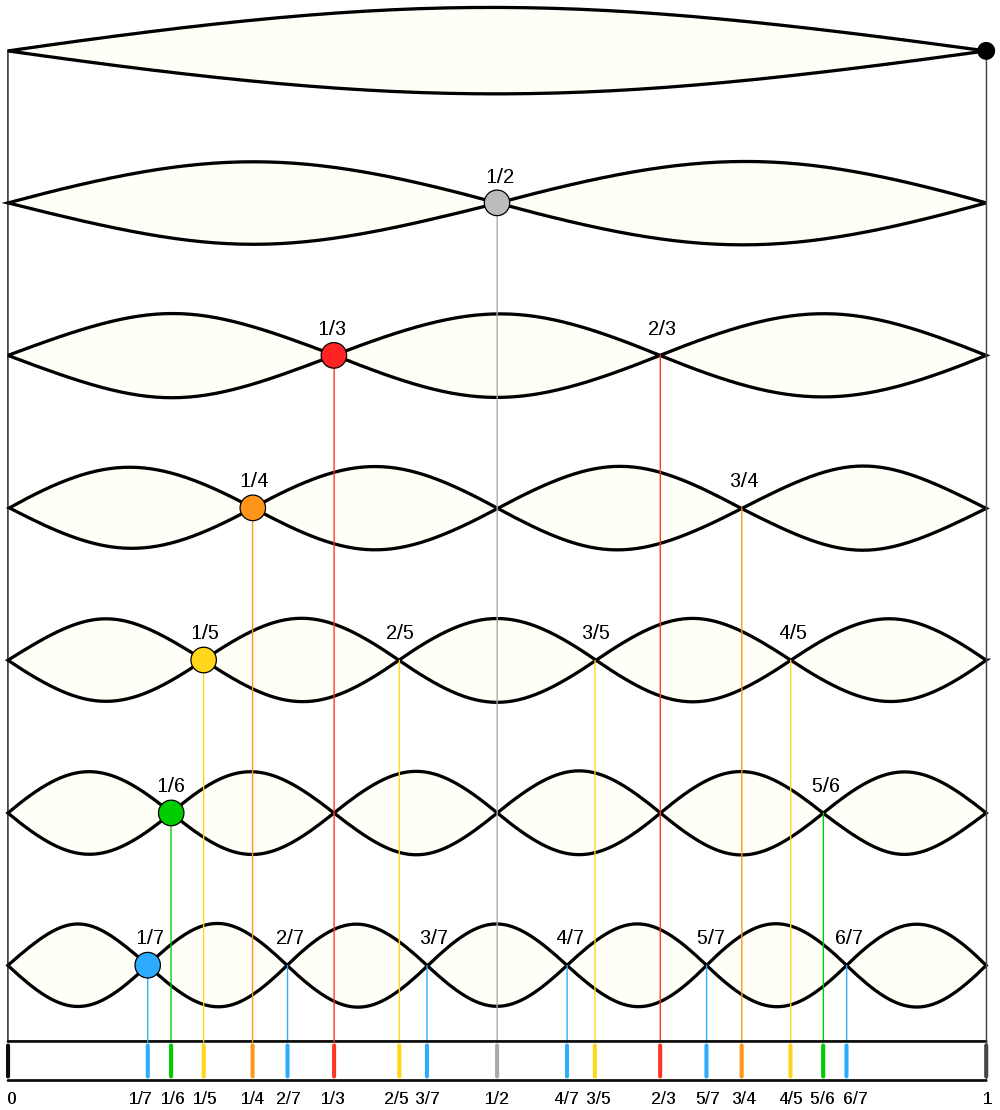
\includegraphics[width=\textwidth,height=0.35\textheight]{img/harmonic-string.png}
\caption{Les harmoniques d'une chorde vibrante}
\end{figure}

Un signal sonore de pitch défini, est une série harmonique de sons purs,
représenté par des ondes sinusoïdales dont les fréquences sont des
multiples \textbf{entiers} d'une fréquence dîte la \textbf{fondamentale}
(où le \textbf{pitch}) notée \(f_0\).

\[ x(t) = \sum\limits_{k\in\mathbb{N}} A_k\cdot\cos(2\pi k f_0 t) \] où
\(A_k\) est l'amplitude de la k\textsuperscript{ème} harmonique.

On cherche donc à indentifier \(f_0\) dans un signal harmonique donnée.

\hypertarget{discretisation-et-echantillonnage}{%
\subsection{Discrétisation et
échantillonnage}\label{discretisation-et-echantillonnage}}

La numérisation d'un signal consiste à prélever des valeurs du signal à
intervalles définis. Les valeurs obtenues sont appelées des
\emph{échantillons}.

La \emph{période d'échantillonnage} \(T_s\) est l'intervalle de temps
entre deux échantillons, on définit \(f_s=\frac{1}{T_s}\) le nombre
d'échantillons prélevés par secondes, \(f_s\) est dît \emph{fréquence
d'échantillonnage} ou en anglais \textbf{sample rate}.

On note \(x[n] = x(t_n)\) où \(t_n = n\cdot T_s = \frac{n}{f_s}\). Dans
le reste du projet, on notera toujours \([\cdot]\) les valeurs
discrètes.

L'échantillonnage d'un signal consiste à choisir une fréquence
d'échantillonnage sans perdre de valeurs importantes du signal. En
traitement de signaux sonores, \(f_s\) est souvent égale à
\(44.1 kHz, 22.05 kHz, 16 kHz,\text{ou } 8kHz\). La numérisation d'un
signal dépend aussi d'autre facteurs comme le \emph{bit depth} (i.e.~le
nombre de bits pour stocker chaque échantillon), mais nous ne nous
intéressons pas par les détails; les bases de l'échantillonnage de
signaux sont expliquées et démontrées par le théroème d'échantillonnage
de \textbf{Nyquist-Shannon}.

\hypertarget{la-transformee-de-fourier-ft}{%
\subsection{La transformée de Fourier
(FT)}\label{la-transformee-de-fourier-ft}}

La transformée de Fourier se définit par:
\[\hat{x}(f) = \int\limits_{-\infty}^{\infty} x(t)\cdot e^{-2\pi j ft}\mathrm{d}t\]

Cette transformation permet d'identifier la fréquence d'une fonction
périodique. En effet, La transformée de Fourier représente l'intensité
d'une fréquence dans un signal, donc ses pics correspondent aux
fréquences du signal.

Comme la transformée de Fourier est linéaire, la transformée d'un signal
harmonique produit plusieurs pics.

\begin{figure}
\centering
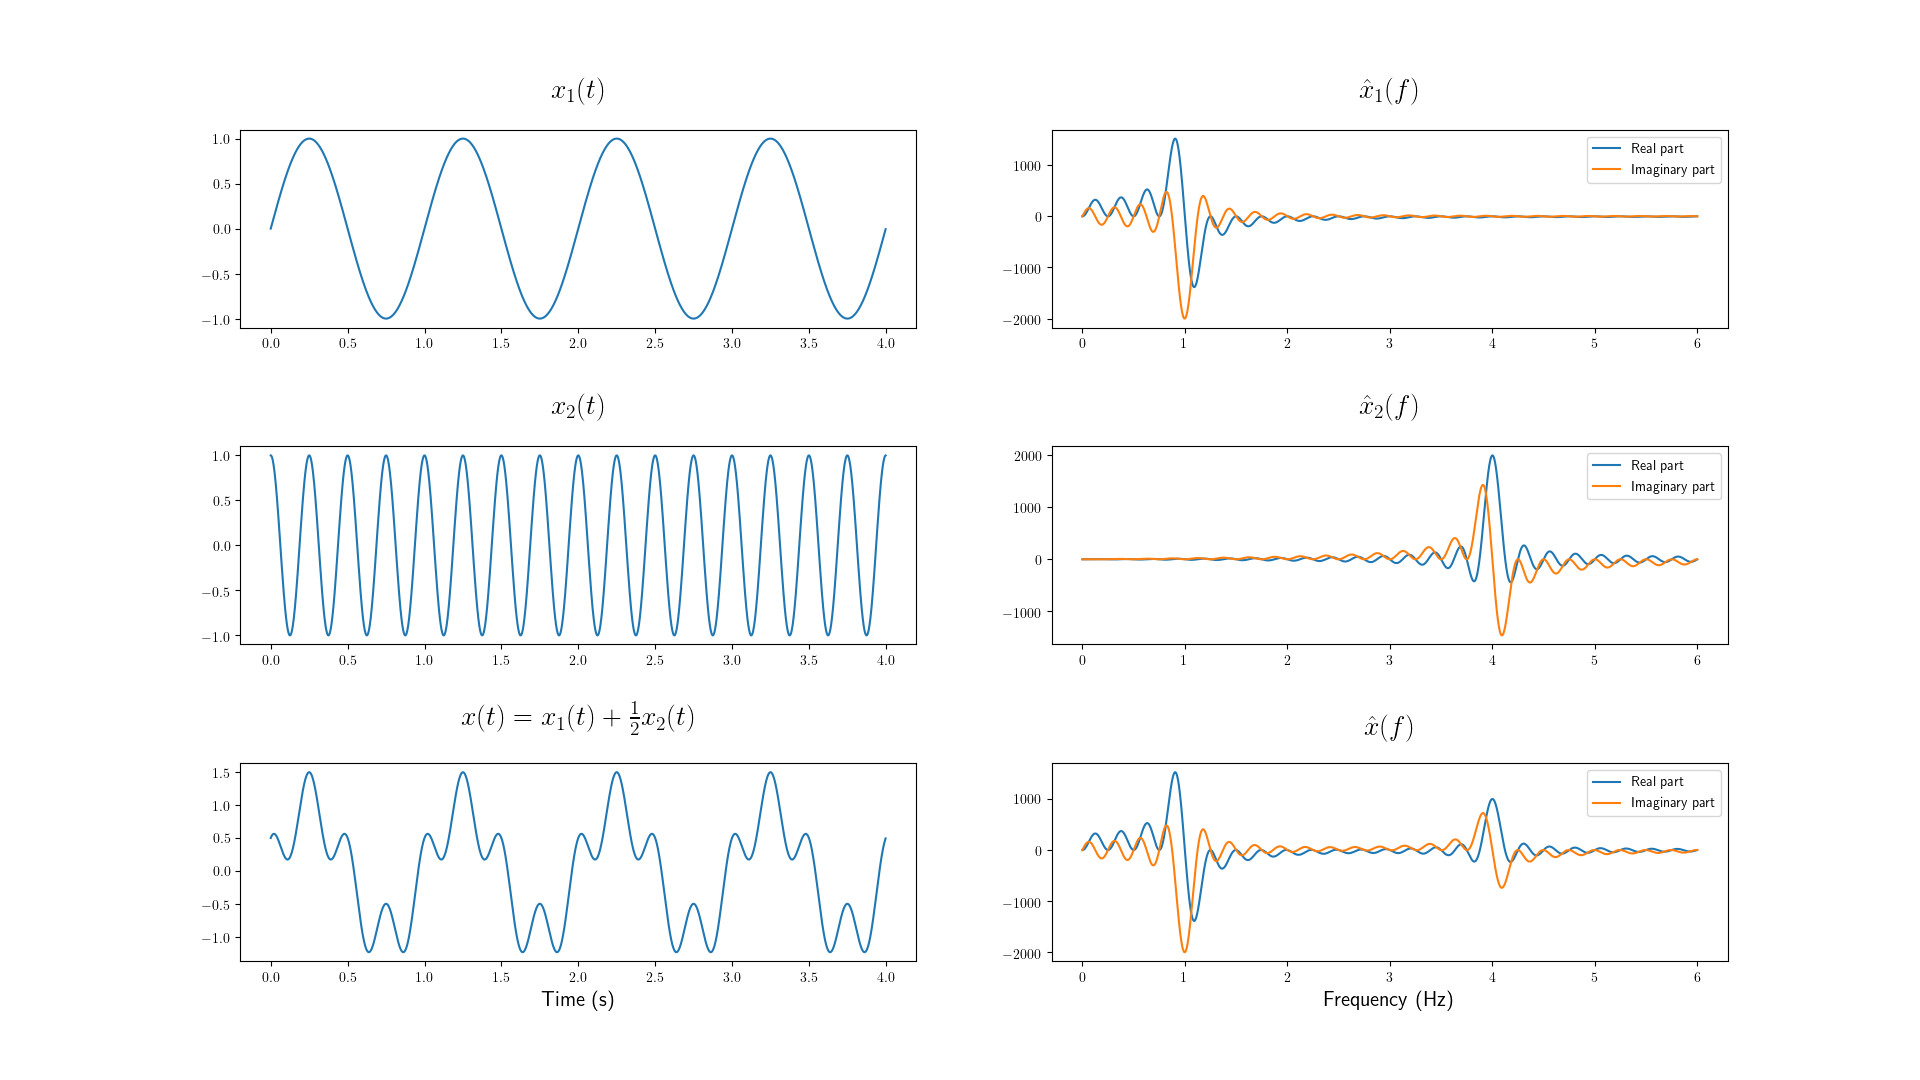
\includegraphics{../../figures/out/fourier_linearity.png}
\caption{Linéarité de la transformée de Fourier}
\end{figure}

\hypertarget{la-transformee-de-fourier-discrete-dft}{%
\subsection{La transformée de Fourier discrète
(DFT)}\label{la-transformee-de-fourier-discrete-dft}}

Soit \(N\) le nombre d'échantillons pris sur l'intervalle
\([0,t_{\text{max}}[\), soit \(f_s\) la fréquence d'échantillonage. Pour
\(n=0,1,\dots,N-1\) on a:

\begin{align*}
\hat{x}(f) &= \int\limits_{0}^{t_{\text{max}}} x(t)\cdot e^{-2\pi j ft}\mathrm{d}t \\
    &= \lim\limits_{f_s\rightarrow\infty} \sum\limits_{n=0}^{N-1} x(t_n)\cdot e^{-2\pi j ft_n}\\
    &= \lim\limits_{f_s\rightarrow\infty} \underbrace{\sum\limits_{n=0}^{N-1} x[n]\cdot e^{-2\pi j f \frac{n}{f_s}}}_{\hat{x}[f]}\\
    &= \lim\limits_{f_s\rightarrow\infty} \hat{x}[f]
\end{align*}

La DFT de \(x[n]\) se définit donc par:
\[ \hat{x}[k] = \sum\limits_{n=0}^{N-1} x[n]\cdot e^{-2\pi j k \frac{n}{f_s}} \]

\textbf{Remarque:} La DFT se calcule souvent matriciellement pour
économiser les calculs. De plus, dans le cas où \(N=2^p,p\in\mathbb{N}\)
on calcule la transformée de Fourier rapide (FFT) qui utilise le
symétrie pour minimiser le nombre de calculs.

\hypertarget{fenetrage}{%
\subsection{Fenêtrage}\label{fenetrage}}

Nous avons souvent besoin de traiter le signal sur une durée limitée, on
définit donc une fonction à support compact \(w\) et on étudie le
produit de convolution du signal avec la fenêtre.

Voici quelques exemples de fenêtres:

\begin{itemize}
\tightlist
\item
  Fonction rectangulaire:
  \[ \mathrm{rect}_{[0,T]}(t) = \begin{cases} 1 &\text{si } t\in[0,T]\\0 &\text{sinon} \end{cases} \]
\item
  Fenêtre Hann:
  \[ w(t) = \sin^2 \left( \frac{\pi t}{T} \right) \cdot\mathrm{rect}_{[0,T]}(t) \]
\item
  Fenêtre Welch (fenêtre parabolique):
  \[ w(t) = 1 - \left( \frac{2t - T}{T} \right) \cdot\mathrm{rect}_{[0,T]}(t) \]
\end{itemize}

Nous avons choisi d'utiliser la fenêtre de Hann dans notre projet car
elle attenue le phénomène \textbf{aliasing} qui rend les signaux
indisntinguables lors de l'échantillonnage.

\[w[n] = \sin^2\left(\frac{\pi n}{N -1}\right)
    = \frac{1}{2}\left(1-\cos\left(\frac{2\pi n}{N -1}\right)\right)\]

\begin{figure}
\centering
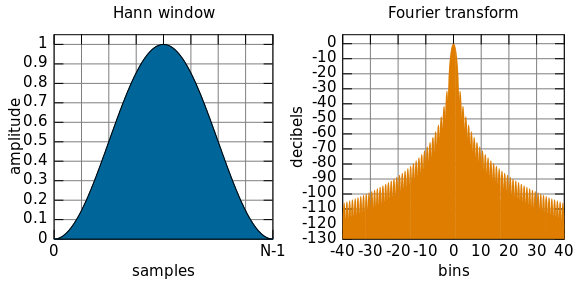
\includegraphics[width=0.7\textwidth,height=\textheight]{img/Hann.png}
\caption{La fenêtre Hann est sa transformée de Fourier}
\end{figure}

\hypertarget{la-transformee-de-fourier-a-court-terme-stft}{%
\subsection{La transformée de Fourier à court terme
(STFT)}\label{la-transformee-de-fourier-a-court-terme-stft}}

La transformée de Fourier nous permet d'obtenir les fréquences d'un
signal harmonique. Or, la fréquence d'un signal peut changer en fonction
du temps, on voudrait donc avoir la transformée de Fourier en fonction
de la fréquence \emph{et} du temps.

La transformée de Fourier à court terme \(X(t,f)\) est la transformée de
Fourier de \(x\) sur une fenêtre glissante \(w\) centrée en \(t\) (i.e.
\(w(\tau-t)\)).

\[X(t, f) = \int\limits_{-\infty}^{\infty} x(\tau)\cdot w(\tau-t)\cdot e^{-2\pi j f\tau} \mathrm{d}\tau \]

De même, la STFT discrète se définit:
\[X[n, k] = \sum\limits_{n=0}^{N-1} x[m]\cdot w[m-n]\cdot e^{-2\pi j k \frac{m}{f_s}}\]

\hypertarget{spectrogramme}{%
\subsection{Spectrogramme}\label{spectrogramme}}

Le spectrogramme permet de visualiser les changement de fréquences en
fonction du temps, il se définit par:
\[ S(t,f) = \left\lvert X(t,f) \right\rvert \]

\textbf{Remarque:} Si on voudrait visualiser la puissance spectrale d'un
signal, on prend le carré de la module de la STFT.

\hypertarget{methodes-danalyse}{%
\subsection{Méthodes d'analyse}\label{methodes-danalyse}}

Ils existent deux types d'analyse de signaux harmoniques:

\begin{enumerate}
\def\labelenumi{\arabic{enumi}.}
\tightlist
\item
  \textbf{Analyse temporelle:} il s'agit d'étudier le signal sans passer
  par la transformée de Fourier.
\item
  \textbf{Analyse fréquentielle/spéctrale:} il s'agit d'étudier le
  spectre du signal (sa transformée de Fourier).
\end{enumerate}

On obtient toujours des meilleurs résultats par l'analyse fréquentielle,
mais la transformée de Fourier demande un calcul coûteux. Dans le cas
d'un signal simple (e.g.~percussion, rythmique, etc) on privilégie
l'analyse temporelle. Sinon, dans le cas d'un signal complexe
(e.g.~instruments mélodiques, signal polyphône, etc) l'analyse
fréquentielle est privilégié.

\hypertarget{implementation}{%
\subsection{Implémentation}\label{implementation}}

On lit un fichier audio grâce à la class \texttt{source} qu'on a défini

\begin{Shaded}
\begin{Highlighting}[]
\ImportTok{from}\NormalTok{ muallef.utils }\ImportTok{import}\NormalTok{ source}
\NormalTok{audio_file }\OperatorTok{=}\NormalTok{ project_path }\OperatorTok{+} \StringTok{"sounds/violin/violin-czardas-cut.wav"}
\NormalTok{sound }\OperatorTok{=}\NormalTok{ source(audio_file)}
\end{Highlighting}
\end{Shaded}

\begin{verbatim}
## /usr/lib/python3.6/site-packages/scipy/io/wavfile.py:273: WavFileWarning: Chunk (non-data) not understood, skipping it.
##   WavFileWarning)
\end{verbatim}

\begin{Shaded}
\begin{Highlighting}[]
\NormalTok{x }\OperatorTok{=}\NormalTok{ sound.signal}
\NormalTok{fs }\OperatorTok{=}\NormalTok{ sound.sampleRate}
\NormalTok{t }\OperatorTok{=}\NormalTok{ sound.get_time()}
\end{Highlighting}
\end{Shaded}

On trace le signal à l'aide de la librairie \texttt{matplotlib}

\begin{Shaded}
\begin{Highlighting}[]
\ImportTok{from}\NormalTok{ matplotlib }\ImportTok{import}\NormalTok{ pyplot }\ImportTok{as}\NormalTok{ plt}
\NormalTok{plt.clf()}
\NormalTok{plt.plot(t, x)}
\NormalTok{plt.show()}
\end{Highlighting}
\end{Shaded}

\includegraphics{index_files/figure-latex/unnamed-chunk-9-1.pdf}

\begin{Shaded}
\begin{Highlighting}[]
\NormalTok{plt.clf()}
\end{Highlighting}
\end{Shaded}

\pagebreak

On trace le spectrogramme du signal

\begin{Shaded}
\begin{Highlighting}[]
\ImportTok{from}\NormalTok{ figures }\ImportTok{import}\NormalTok{ plot_spectrogram}
\NormalTok{fig }\OperatorTok{=}\NormalTok{ plt.figure()}
\NormalTok{ax }\OperatorTok{=}\NormalTok{ fig.add_subplot(}\DecValTok{111}\NormalTok{)}
\NormalTok{ax, out }\OperatorTok{=}\NormalTok{ plot_spectrogram(signal}\OperatorTok{=}\NormalTok{x, sample_rate}\OperatorTok{=}\NormalTok{fs, axis}\OperatorTok{=}\NormalTok{ax, color_map}\OperatorTok{=}\StringTok{'inferno'}\NormalTok{)}
\NormalTok{plt.show()}
\end{Highlighting}
\end{Shaded}

\includegraphics{index_files/figure-latex/unnamed-chunk-10-1.pdf}

\begin{Shaded}
\begin{Highlighting}[]
\NormalTok{plt.clf()}
\end{Highlighting}
\end{Shaded}

\hypertarget{pitch}{%
\section{Pitch}\label{pitch}}

Dans cette partie, nous allons étudier des méthodes de reconnaissance de
la fréquence fondamentale d'un signal.

\hypertarget{yin}{%
\subsection{YIN}\label{yin}}

L'algorithme de YIN \emph{(Kawahara and Cheveigné 2002)} est une méthode
robuste pour la reconnaissance du pitch dans le domaine temporel. Son
principe est la séléction de fréquences candidates parmi toutes les
fréquences détéctées sur l'intervalle de fenêtrage.

La méthode propose que l'expression \(x(t)-x(t+\tau)\) atteint son
minimum quand \(\tau\) est égale à la période du signal (i.e.
\(\frac{1}{f_0}\)). En diffinissant la fonction de différence à
l'instant \(t\) fixé:

\[ d_t[\tau] = \sum\limits_{i=t+1}^{t+W} \left(x[t]-x[t+\tau]\right)^2 \]
où \(W\) est la taille de la fenêtre \(w\), on appelle \(\tau\) le
\emph{retard} (anglais: \emph{lag}).

Par la suite, on calcule la fonction de la moyenne cumulative définie
par: \[d_t'[\tau] = \begin{cases} 1 &\text{si} \tau = 0\\
d_t[\tau] / \frac{1}{\tau}\sum\limits_{i=0}^{\tau}d_t[i] &\text{sinon}
\end{cases}\]

Les candidats sont les minimums locaux de \(d_t'\). On séléctionne les
candidats avec \(d_t'[\tau]\) inférieur à un seuil fixé (les auteurs
recommandent un seuil de 0.1).

\hypertarget{yin-spectrale}{%
\subsection{YIN spectrale}\label{yin-spectrale}}

L'algorithme de YIN spectrale \emph{(Brossier 2007)} est une méthode qui
utilise la même logique de l'algorithme de YIN et l'applique sur le
spectre du signal.

La fonction de différence est définie par le carré de la différence
spéctrale: \begin{align*}
\hat{d}_t[\tau] &= \frac{4}{N} \sum\limits_{k=0}^{\frac{N}{2}+1} \left\lvert X[t,k] \right\rvert^2
       - \frac{2}{N} \sum\limits_{k=0}^{\frac{N}{2}+1} \left\lvert X[t,k] \right\rvert^2
       \cdot \cos \left( \frac{2\pi k\tau}{N} \right) \\
    &= \frac{2}{N} \sum\limits_{k=0}^{\frac{N}{2}+1} \left\lvert X[t,k] \right\rvert^2
       \cdot \left( 2 - \cos \left( \frac{2\pi k\tau}{N} \right) \right) \\
    &= \frac{2}{N} \sum\limits_{k=0}^{\frac{N}{2}+1}
       \left\lvert\left( 1-e^{2\pi jk\tau/N} \right) X[t,k] \right\rvert^2
\end{align*}

La fonction de la moyenne cumulative se calcule de façon analogue à
l'algorithme de YIN. L'algorithme cherche le minimum globale de cette
dernière.

Cette méthode est la plus utilisée pour la détection de pitch car elle
donne de très bonnes résultats et a pour complixité \(O(n\log n)\)

\hypertarget{implementation-1}{%
\subsection{Implémentation}\label{implementation-1}}

\begin{Shaded}
\begin{Highlighting}[]
\ImportTok{import}\NormalTok{ numpy }\ImportTok{as}\NormalTok{ np}
\ImportTok{from}\NormalTok{ muallef }\ImportTok{import}\NormalTok{ pitch}
\NormalTok{t, f, conf }\OperatorTok{=}\NormalTok{ pitch.detect(signal}\OperatorTok{=}\NormalTok{x, sampleRate}\OperatorTok{=}\NormalTok{fs, bufferSize}\OperatorTok{=}\DecValTok{2048}\NormalTok{, method}\OperatorTok{=}\StringTok{'yinfft'}\NormalTok{)}
\CommentTok{# t: le temps en secondes}
\CommentTok{# f: la fréquence en Hz}
\CommentTok{# conf: le taux de confiance}
\NormalTok{size }\OperatorTok{=}\NormalTok{ np.power(conf, }\DecValTok{3}\NormalTok{)}
\NormalTok{fig }\OperatorTok{=}\NormalTok{ plt.figure()}
\NormalTok{ax }\OperatorTok{=}\NormalTok{ fig.add_subplot(}\DecValTok{111}\NormalTok{, ylim}\OperatorTok{=}\NormalTok{(}\DecValTok{170}\NormalTok{, }\DecValTok{600}\NormalTok{))}
\NormalTok{ax.scatter(t, f, marker}\OperatorTok{=}\StringTok{'o'}\NormalTok{, s}\OperatorTok{=}\NormalTok{size)}
\NormalTok{ax.set_xlabel(}\StringTok{"Time (s)"}\NormalTok{)}
\NormalTok{ax.set_ylabel(}\StringTok{"Frequency (Hz)"}\NormalTok{)}
\NormalTok{plt.show()}
\end{Highlighting}
\end{Shaded}

\includegraphics{index_files/figure-latex/unnamed-chunk-11-1.pdf}

\begin{Shaded}
\begin{Highlighting}[]
\NormalTok{plt.clf()}
\end{Highlighting}
\end{Shaded}

\pagebreak

\hypertarget{segmentation-temporelle}{%
\section{Segmentation temporelle}\label{segmentation-temporelle}}

L'étape fondamentale dans la reconnaissance du son est la segmentation
temporelle. Il s'agit de trouver les frontières des objets sonores,
c'est-à-dire:

\begin{itemize}
\tightlist
\item
  Le début de la note -- dît \textbf{\emph{onset}}.
\item
  La fin de la note -- dît \textbf{\emph{offset}}.
\end{itemize}

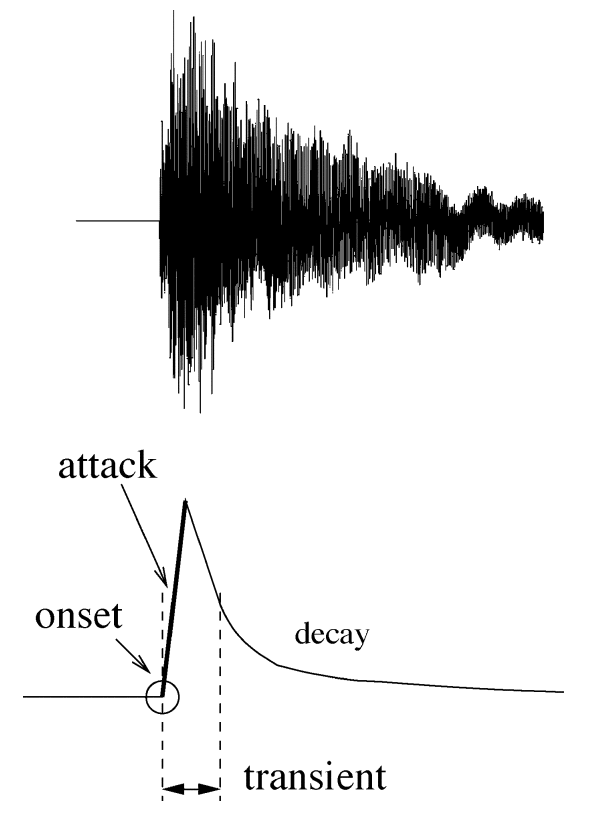
\includegraphics[width=0.5\textwidth,height=\textheight]{img/onset.png}

Attack, transient, decay, onset IEEE TRANSACTIONS ON SPEECH AND AUDIO
PROCESSING, VOL. 13, NO. 5, SEPTEMBER 2005

Cette étape dépend fortement sur le type du son produit; les instrument
à chordes pincées (guitare, piano, oud, etc.) ont un profile différent
de celui des instruments à cordes frottées (la famille du violon) ou de
celle des instruments à vent.

Dans cette partie on expliquera les méthodes implémentés pour la
reconnaissance du \textbf{onset}.

\hypertarget{methode}{%
\subsection{Méthode}\label{methode}}

La lecture scientifique nous a donné une méthode rigoureuse qu'on a
simplifié pour obtenir des résultats rapidement.

Il s'agit de définir une fonction qui permet de quantifier la
perturbation du signal à un moment donné, cette fonction est souvent
appelée \textbf{Onset Detection Function} ou \textbf{Onset Strength
Signal}, dans ce projet on fera référence à cette dernière par
\textbf{Onset Detection Function} ou \textbf{\emph{ODF}}.

Théoriquement, les maximums locaux de l'ODF sont les onsets du signal,
mais en pratique il s'agit d'un sous-ensemble de ces points. En effet,
l'ODF est souvent très sensible et détectera la moindre des
perturbations.

Ce problème pourra être résolu en définissant un seuil au dessous duquel
aucun onset est considéré. Ils existent plusieurs méthodes pour définir
tel seuil.

Soit un seuil fixe, ce qui minimise le coût des calculs au prix de la
qualité des résultats. Soit de calculer un seuil variable, il s'agit de
lisser la fonction ODF par des méthodes classiques comme la moyenne
mobile.

La méthode consiste donc en trois étapes:

\begin{enumerate}
\def\labelenumi{\arabic{enumi}.}
\tightlist
\item
  Calcul de l'\textbf{Onset Detection Function}.
\item
  \textbf{Thresholding}: calcul du seuil.
\item
  \textbf{Peak-picking}: la selection des onsets.
\end{enumerate}

Une méthode heuristique est proposée par (Rosão, Ribeiro, and Matos
2012) pour séléctionner les onsets, il s'agit de trouver les points
\(t_n\) tels que, pour \(a,b,\tau\in\mathbb{N}, \delta\in{R_+}\) fixés:
- \(x[n] = \max\limits_{n+a \leq i\leq n + b} x[i]\) -
\(x[n] \geq \delta + \frac{1}{a+b+1}\sum\limits_{n+a \leq i\leq n + b} x[i]\)
- Si \(O\) est l'ensembles d'onsets,
\(\forall n,m\in O, \lvert n - m \rvert > \tau\)

Cette méthode permet de vérifier que le point choisi est un maximum
local et suffisament loin du point précédant, l'avantage de cette
méthode est sa rapidité.

\hypertarget{onset-detection-function-odf}{%
\subsection{Onset Detection Function
(ODF)}\label{onset-detection-function-odf}}

Ils existent plusieurs fonction de détéction d'onsets, on expliquera
quelques unes qui se basent sur la STFT.

\hypertarget{high-frequency-content-hfc}{%
\subsubsection{High Frequency Content
(HFC)}\label{high-frequency-content-hfc}}

Il s'agit de priviligier les fréquences élevées dans un signal.
\[ D_{HFC}[n] = \sum\limits_{k=1}^{N}k\cdot\left\lvert X[n,k]\right\rvert^2 \]
(Masri 1996)

\hypertarget{phase-deviation-phi}{%
\subsubsection{Phase Deviation (Phi)}\label{phase-deviation-phi}}

Il s'agit de calculer les différences de phases en dérivant l'argument
complex de la STFT, on note \[ \varphi(t, f) = \mathrm{arg}(X(t, f)) \]
\[\hat{\varphi}(t, f) = \mathrm{princarg}
\left( \frac{\partial^2 \varphi}{\partial t^2}(t, f)  \right) \] où
\[ \mathrm{princarg}(\theta) = \pi + ((\theta + \pi) mod (-2\pi)) \]
donc la ODS de phase se calcule par la formule:
\[ D_{\Phi}[n] = \sum\limits_{k=0}^{N}\left\lvert \hat{\varphi}[n, k] \right\rvert \]
(Bello and Sandler 2003)

Dans notre implémentation, nous avons approximé la dérivée partielle
seconde de la phase par un schéma de Taylor d'ordre 2.

\hypertarget{complex-distance}{%
\subsubsection{Complex Distance}\label{complex-distance}}

Cette méthode permet de qualifier les changements spectraux du signal
ainsi que les changements en phase. Il s'agit de calculer une prédiction
du spectre du signal, et puis le comparer par sa valeur. On reprend la
fonction calculée en \(\hat{varphi}(t, f)\) de la méthode précédante. On
définit la prédiction :
\[ \hat{X}[n, k] = \left\lvert X[n, k] \right\rvert \cdot e^{j\hat{\varphi}[n, k]} \]

Donc la distance complexe se calcule:
\[ D_{\mathbb{C}}[n] = \sum\limits_{k=0}^{N} \left\lvert  \hat{X}[n, k] - X[n, k] \right\rvert ^2 \]
(Duxbury et al. 2003)

\hypertarget{thresholding}{%
\subsection{Thresholding}\label{thresholding}}

Nous avons décidé de lisser la fonction ODF par une moyenne mobile
echelonnées par la fenêtre Hann, il s'agit du produit de convolution de
l'ODF avec la fonction Hann.

\hypertarget{resultats}{%
\subsection{Résultats}\label{resultats}}

Au premier lieu, nous avons effectués des tests sur des morceaux de
violon joués par Rand et nous avons obtenus de très mauvaises résultats
de segmentation temporelle. Nous avons ensuite essayé des morceaux plus
facile joués par des musiciens plus expérimentés mais nous n'avons pas
obtenu des meilleurs résultats.

On a donc considéré d'autres instruments, nottamment ceux à chordes
pincées comme le piano et la guitare. Nous avons directement obtenu des
très bons résultats.

Ceci s'explique par le fait que la famille de violon (chordes frottées)
produit un son \textbf{\emph{Legato}}, la segmentation temporelle dépend
donc moins sur l'énergie du signal (ou son spectre) et plus sur la
fréquence fondamentale.

\begin{figure}
\centering
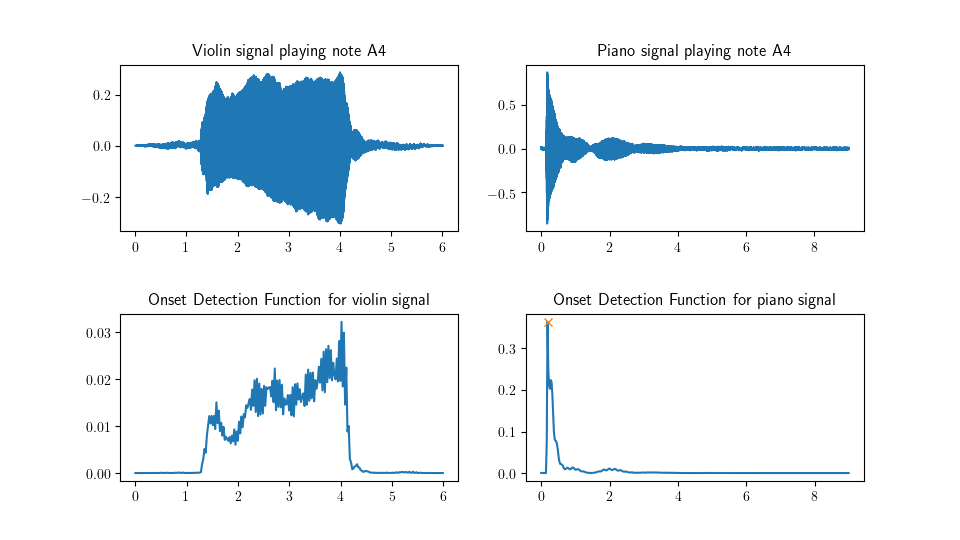
\includegraphics{../../figures/out/onset.png}
\caption{Comparaison entre les profiles temporels du violon et du piano}
\end{figure}

On voit bien que les onsets sont bien détectés dans le cas du piano.
Voici le morceau fameux de Beethoven \textbf{Für Elise}.

\begin{Shaded}
\begin{Highlighting}[]
\ImportTok{from}\NormalTok{ muallef.onset }\ImportTok{import}\NormalTok{ onset_function}
\ImportTok{from}\NormalTok{ muallef.onset.peak_picker }\ImportTok{import}\NormalTok{ peak_pick}
\NormalTok{piano_sound }\OperatorTok{=}\NormalTok{ project_path }\OperatorTok{+} \StringTok{"sounds/piano/FurElise-mono.wav"}
\NormalTok{fur_elise }\OperatorTok{=}\NormalTok{ source(piano_sound)}
\end{Highlighting}
\end{Shaded}

\begin{verbatim}
## /usr/lib/python3.6/site-packages/scipy/io/wavfile.py:273: WavFileWarning: Chunk (non-data) not understood, skipping it.
##   WavFileWarning)
\end{verbatim}

\begin{Shaded}
\begin{Highlighting}[]
\NormalTok{plt.clf()}
\NormalTok{fig }\OperatorTok{=}\NormalTok{ plt.figure()}
\NormalTok{ax1 }\OperatorTok{=}\NormalTok{ fig.add_subplot(}\DecValTok{211}\NormalTok{)}
\NormalTok{ax1.plot(fur_elise.get_time(), fur_elise.signal)}
\NormalTok{ax1.set_title(}\StringTok{"Piano signal"}\NormalTok{)}
\NormalTok{ax2 }\OperatorTok{=}\NormalTok{ fig.add_subplot(}\DecValTok{212}\NormalTok{)}
\NormalTok{t, odf }\OperatorTok{=}\NormalTok{ onset_function(signal}\OperatorTok{=}\NormalTok{fur_elise.signal, sampleRate}\OperatorTok{=}\NormalTok{fur_elise.sampleRate,}
\NormalTok{                                windowSize}\OperatorTok{=}\DecValTok{2048}\NormalTok{, method}\OperatorTok{=}\StringTok{"complex"}\NormalTok{, normalize}\OperatorTok{=}\VariableTok{True}\NormalTok{)}
\NormalTok{ax2.plot(t, odf, label}\OperatorTok{=}\StringTok{"Complex Distance"}\NormalTok{)}
\NormalTok{onsets }\OperatorTok{=}\NormalTok{ peak_pick(odf, delta}\OperatorTok{=}\FloatTok{0.05}\NormalTok{, wait}\OperatorTok{=}\DecValTok{4}\NormalTok{)}
\NormalTok{ax2.plot(t[onsets], odf[onsets], marker}\OperatorTok{=}\StringTok{"x"}\NormalTok{, ls}\OperatorTok{=}\StringTok{""}\NormalTok{, label}\OperatorTok{=}\StringTok{"Peaks"}\NormalTok{)}
\NormalTok{ax2.legend(loc}\OperatorTok{=}\StringTok{"upper right"}\NormalTok{)}
\NormalTok{ax2.set_title(}\StringTok{"Onset Detection Function & Selected Peaks"}\NormalTok{)}
\NormalTok{plt.subplots_adjust(hspace}\OperatorTok{=}\FloatTok{0.5}\NormalTok{)}
\NormalTok{plt.show()}
\end{Highlighting}
\end{Shaded}

\includegraphics{index_files/figure-latex/unnamed-chunk-12-1.pdf}

\pagebreak

\hypertarget{theorie-de-musique}{%
\section{Théorie de musique}\label{theorie-de-musique}}

La théorie de la musique permet, à la fois de réglementer la musique et
de la libéraliser.

\hypertarget{notions-de-base}{%
\subsection{Notions de base}\label{notions-de-base}}

La \textbf{note} est le plus petit objet musical, porte un nom, et
caractérise la hauteur tonal du son (fréquence). Dans le contexte d'un
morceau musical, une note caractérise aussi la durée de cet objet.

Un \textbf{intervalle} se définit musicalement par l'écart de hauteur
tonal entre deux notes. Scientifiquement, un intervalle est le ratio de
fréquences fondamentales de deux notes.

On appelle \textbf{\emph{octave}} l'intervalle correspondant au ratio
\(2:1\) Les notes d'un octave porte le même nom.

Une \textbf{échelle} musicale est une suite d'intervalles conjoints. Une
\textbf{gamme} musicale est une suite de notes conjointes, la dernière
répétant la première à l'octave.

L'\textbf{armure} --- ou l'\textbf{armature} (\emph{en:} \textbf{key
signature}) --- est un ensemble d'altérations réunies à la clé. Elle est
composée soit exclusivement de dièses, soit exclusivement de bémols ---
en dehors du cas particulier constitué par le changement d'armure. Ces
altérations correspondent à la tonalité principale des mesures suivant
la clé.

Ils existent plusieurs théories de musique qui diffèrent principalement
par la composition d'échelles et de gammes. Dans ce projet nous avons
considéré la théorie de la musique occidentale basée sur l'accord
tempéré.

\hypertarget{tonalite}{%
\subsection{Tonalité}\label{tonalite}}

\hypertarget{generalites}{%
\subsubsection{Généralités}\label{generalites}}

\begin{itemize}
\tightlist
\item
  L'unité de tonalité est le \textbf{\emph{ton}}.
\item
  En musique classique, le plus petit intervalle est d'un
  \textbf{\emph{demi-ton}}.
\item
  Un octave est composée de 6 tons, soit 12 demi-tons.
\item
  L'échelle majeure classique est composée des intervalles:
  1--1--½--1--1--1--½.
\item
  La gamme majeure classique est composée de 7 notes distinctes (la
  8\textsuperscript{ème} est à l'octave de la première).
\item
  \textbf{Le dièse (\#)} est une altération qui lève une note d'un
  demi-ton.
\item
  \textbf{Le bémol (\(\flat\))} est une altération qui baisse une note
  d'un demi-ton.
\end{itemize}

\hypertarget{les-notes}{%
\subsubsection{Les notes}\label{les-notes}}

Les notes principales sont les touches blanches d'un piano. Les touches
noirs d'un piano sont des notes altérées.

\begin{itemize}
\tightlist
\item
  Noms français: do-ré-mi-fa-sol-la-si
\item
  Noms alphabétiques: C-D-E-F-G-A-B
\end{itemize}

\textbf{Remarque:} Certaines notes altérées sont des touches blanches
(e.g.~Mi\#=Fa\(\equiv\)touche blanche), sans détailler sur les
altérations composées (doubles dièses, doubles bémols).

\hypertarget{nomenclature}{%
\subsubsection{Nomenclature}\label{nomenclature}}

Ils existent plusieurs systèmes de nomenclature de notes de musique. Le
système utilisé en France adopte les noms en termes de
\emph{Do-Ré-Mi-Fa-Sol-La-Si}. De plus, il existe un système basé sur
l'alphabet latin : \emph{C-D-E-F-G-A-B}. Les deux systèmes sont très
utilisés, dans ce projet on utilisera le dernière pour simplifier.

Vu que les noms des notes se répètent au bout d'un octave, il faut
distinguer une note \emph{LA} de fréquence \(440Hz\) d'une autre de
fréquence \(220Hz\) ou \(880Hz\).

Le système de notation scientifique \textbf{Scientific Pitch Notation}
identifie une note par sont nom alphabetique avec un nombre identifiant
l'octave dans laquelle elle se situe, où l'octave commence par une note
\emph{C}. Par exemple la fréquence \(440Hz\) représente \(A_4\) sans
ambiguité, et les fréquences \(220Hz\) et \(880Hz\) représentent les
notes \(A_3, A_5\) respectivement.

Dans le protocole \textbf{MIDI}, le notes sont représentées par un
nombre entier, il permet de coder plus de 10 octave en partant de la
note \(C_{-1}\).

\begin{figure}
\centering
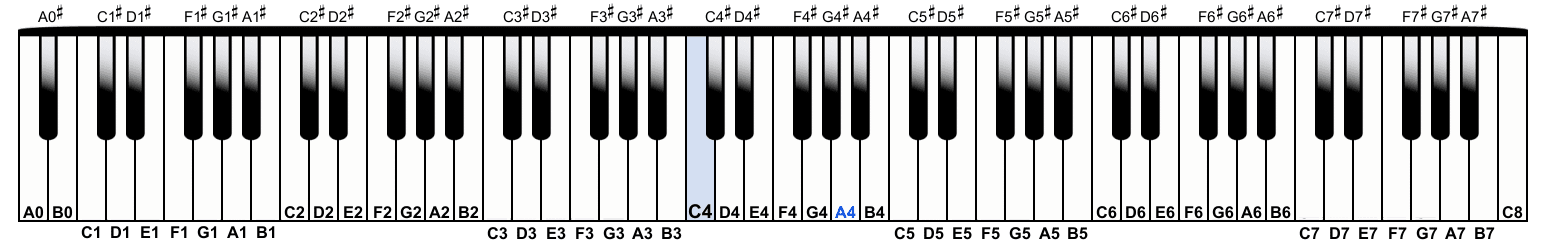
\includegraphics[width=1\textwidth,height=\textheight]{img/piano-keys.png}
\caption{La notation scientifique sur un piano}
\end{figure}

\hypertarget{les-gammes-classiques}{%
\subsubsection{Les gammes classiques}\label{les-gammes-classiques}}

À chaque tonalité majeure est associée une tonalité en mode mineur,
présentant la même armure de clef et appelée relative mineure.

\begin{figure}
\centering
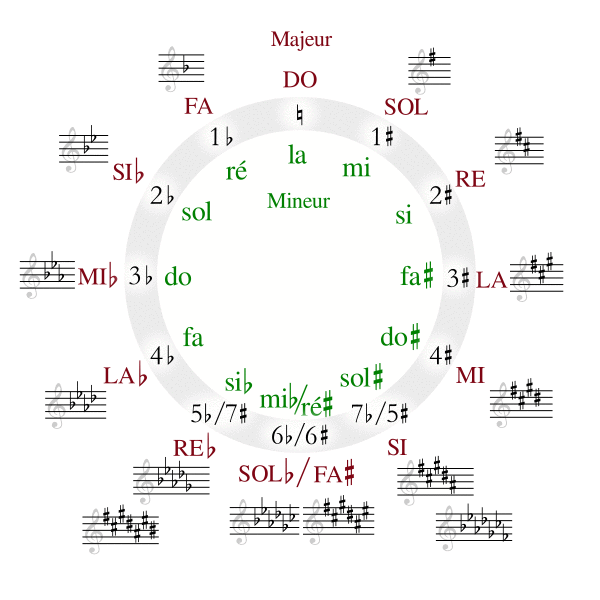
\includegraphics[width=0.5\textwidth,height=\textheight]{img/cycle-des-quintes.png}
\caption{Le cycle des quintes}
\end{figure}

Pour simplifier, on va considérer la théorie de la musique occidentale
basée sur l'accord tempéré (depuis le XVIII\textsuperscript{e} siècle).
Dans ce cas, l'intervalle séparant la première et la dernière note d'une
gamme est dite \emph{octave}, une octave se divise en 12 écarts égales
appelés \emph{demi-tons}. La dernière note porte le même nom de la
première dans la gamme.

\begin{figure}
\centering
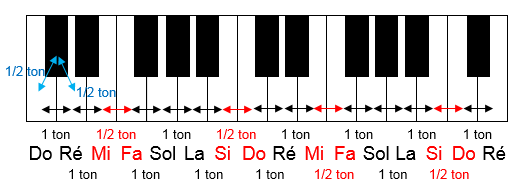
\includegraphics[width=1\textwidth,height=\textheight]{img/intervalles-piano.png}
\caption{Les intervalles sur un piano}
\end{figure}

\hypertarget{tonalites-frequences}{%
\subsection{Tonalités \& Fréquences}\label{tonalites-frequences}}

L'espace de notes est un espace linéaire discrèt, mais l'espace de
fréquences est continue non-linéaire. Par exemple, la l'intervalle entre
A3 et A4 est un octave, celui entre A4 et A5 également. En revanche,
\(f(A3)=220Hz, f(A4)=440Hz, f(A5)=880Hz\), on voit bien que la relation
est logarithmique. Le problème consiste à trouver une fonction qui
associe les fréquences fondamentales obtenues avec des valeurs entières.

\hypertarget{le-protocole-midi}{%
\subsubsection{Le protocole MIDI}\label{le-protocole-midi}}

On voudrais savoir le rapport \(r\) de fréquences associé à un demi-ton,
sachant que l'octave double la fréquence on peut conclure facilement:
\[ r^{12} = 2 \Rightarrow r=2^{1/12} \]

On souhaite ramener l'espace de fréquences \((\mathbb{R},\times)\) à
l'espace \((\mathbb{N},+)\) tel que \(\boxed{\text{demi-ton}\equiv 1}\).
On définit donc une bijection
\[\forall f\in]0,\infty[, f\mapsto 12 \log_2 f \] En arrondissant le
résultat à la valeur entière la plus proche, on obtient un espace
linéaire discrèt correspondant aux notes.

Il sera convenient d'obtenir les mêmes notes du protocole \textbf{MIDI}
vu qu'il est très bien établi et très utilisé. Pour cela, on effectue
une petite translation, en partant de la note de référence
\(A4\equiv 69_{\text{MIDI}} \equiv 440Hz\).

\[\begin{cases}
\varphi:f\mapsto 12\log_2 f + c_{\text{ref}}\\
\varphi(440) = 69
\end{cases}\Rightarrow c_{\text{ref}} = 69 - 12\log_2 440\] Par
conséquent, la bijection \(\varphi\) est définit par :
\[\varphi: ]0,\infty[ \rightarrow \mathbb{R} : f \mapsto 12\log_2 f + c_{\text{ref}}
\quad\text{avec } c_{\text{ref}}=69 - 12\log_2 440\] On note
\(\bar{\varphi}\) la fonction définit par
\(\bar{\varphi}(f)=\left\lfloor\varphi(f)\right\rceil\in\mathbb{Z}\) où
\(\lfloor\cdot\rceil\) est la fonction d'arrondissement à l'entier le
plus proche.

On peut donc obtenir les nombres MIDI de notes à partir des fréquences
fondamentales grâce à la fonction \(\bar{\varphi}\).

Néanmoins, le nombre MIDI n'est pas suffisant pour identifier une note,
car certaines notes ont la même fréquence en accord tempéré et donc le
même nombre midi (i.e.~la même touche sur un piano), par exemple
\(\text{MIDI}(C\#)=\text{MIDI}(D\flat)\). Pour distinguer ces notes il
est nécessaire de trouver la gamme du morceau.

\hypertarget{reconnaissance-de-la-gammelarmature}{%
\subsection{Reconnaissance de la
gamme/l'armature}\label{reconnaissance-de-la-gammelarmature}}

Dans cette étude, on ne s'intéressera aux notes dans une octave. On
introduit donc la fonction \(\psi\) :
\[\psi: ]0,\infty[ \rightarrow [0,12[ : f \mapsto \psi(f) \mod 12\] De
même, on définit la fonction \(\bar{\psi}\) telle que
\(\bar{\psi}(f)=\left\lfloor\psi(f)\right\rceil\). On voit que
\(\mathrm{Im}(\bar{\psi})=\mathbb{Z}/12\mathbb{Z}\).

\vspace{-1em}

\begin{longtable}[]{@{}lcccccccccccc@{}}
\toprule
Note & C & & D & & E & F & & G & & A & & B\tabularnewline
\midrule
\endhead
\(\bar{\psi}(f)\) & 0 & 1 & 2 & 3 & 4 & 5 & 6 & 7 & 8 & 9 & 10 &
11\tabularnewline
\bottomrule
\end{longtable}

En musique classique, ils existent 4 types de gammes, on ne
s'intéressera qu'à un : \emph{la gamme majeure}. Comme on l'a déjà dit,
une gamme est caractérisée par sa première note et la suite des
intervalles. Dans la gamme majeure, les intérvalles en fonction du ton
sont : 1--1--½--1--1--1--½.

La gamme \emph{Do/C Majeur} contient donc les notes \{0, 2, 4, 5, 7, 9,
11\}.

De même, la gamme \emph{Sol/G Majeur} contient les notes \{7, 9, 11, 0,
2, 4, 6\}. Ces gammes diffèrent par une note, la note 5\(\equiv\)F est
remplacée par la note 6 qui correspond à F\# ou G\(\flat\). Dans le
contexte du Sol Majeur, on sait que 6\(\equiv\)F\# car la gamme contient
déjà 7\(\equiv\)G.

On voit bien que l'identification de la gamme est \emph{nécessaire} pour
la distinction entre certaines notes.

Une gamme peut être alors identifié par son ensemble de notes qu'on
notera \(G\) tel que \(G\subset\mathbb{Z}/12\mathbb{Z}, |G|=7\). On
définit le vecteur \(g\in\left\{0,1\right\}^{12}\) associé à \(G\) tel
que \[ g_i = 1_G(i) =
\begin{cases} 1 & \text{si } i\in G\\ 0 &\text{sinon}\end{cases}\] On
définit donc \(E\) l'ensemble de gammes majeures.

Soit \(F\) l'ensemble de fréquences fondamentales obtenues, soit
\(S=\bar{\psi}(F)\subset\mathbb{Z}/12\mathbb{Z}\).

On définit
\(p:{Z}/12\mathbb{Z}\rightarrow\mathbb{N}:n\mapsto\text{le nombre d'occurances de $n$ dans le morceau}\).

On note \(p_{\max}=\max\limits_{n\in S} p(n)\). On définit le vecteur
\(x\in\left[0,1\right]^{12}\) tel que \(x_i=\frac{p(i)}{p_{\max}}\).

La gamme du morceau est alors la solution du problème d'optimisation
\[ \min\limits_{g\in E}\quad \lVert g-x \rVert \] En musique classique,
\(\lvert E\rvert = 12\) donc le problème d'optimisation ne nécessite pas
une résolution mathémtique avancée.

\hypertarget{implementation-2}{%
\subsection{Implémentation}\label{implementation-2}}

Nous pouvons tester cet algorithme sur notre morceau:

\begin{Shaded}
\begin{Highlighting}[]
\ImportTok{from}\NormalTok{ muallef.utils.units }\ImportTok{import}\NormalTok{ convertFreq}
\ImportTok{from}\NormalTok{ muallef.notes }\ImportTok{import}\NormalTok{ scale, name}
\ImportTok{from}\NormalTok{ muallef.utils.io }\ImportTok{import}\NormalTok{ plot_step_function}
\NormalTok{midi }\OperatorTok{=}\NormalTok{ convertFreq(f, }\StringTok{"Hz"}\NormalTok{, }\StringTok{"MIDI"}\NormalTok{)}
\NormalTok{plt.clf()}
\NormalTok{fig }\OperatorTok{=}\NormalTok{ plt.figure()}
\NormalTok{ax }\OperatorTok{=}\NormalTok{ fig.add_subplot(}\DecValTok{111}\NormalTok{, ylim}\OperatorTok{=}\NormalTok{(}\DecValTok{50}\NormalTok{,}\DecValTok{80}\NormalTok{))}
\NormalTok{plot_step_function(t, midi)}
\NormalTok{plt.show()}
\end{Highlighting}
\end{Shaded}

\includegraphics{index_files/figure-latex/unnamed-chunk-13-1.pdf}

\begin{Shaded}
\begin{Highlighting}[]
\NormalTok{base_note }\OperatorTok{=}\NormalTok{ scale.detect_scale(midi)}
\NormalTok{nb_alt, tone }\OperatorTok{=}\NormalTok{ scale.scale_signature(base_note)}
\BuiltInTok{print}\NormalTok{(}\StringTok{"Major scale: "}\NormalTok{, name.octave_note_name(base_note, tone))}
\end{Highlighting}
\end{Shaded}

\begin{verbatim}
## Major scale:  Fa
\end{verbatim}

\begin{Shaded}
\begin{Highlighting}[]
\NormalTok{key_signature }\OperatorTok{=} \StringTok{""}
\ControlFlowTok{if}\NormalTok{ tone }\OperatorTok{>} \DecValTok{0}\NormalTok{:}
    \ControlFlowTok{for}\NormalTok{ i }\KeywordTok{in} \BuiltInTok{range}\NormalTok{(nb_alt):}
\NormalTok{        key_signature }\OperatorTok{+=}\NormalTok{ name.octave_note_name(scale.sharp[i], tone) }\OperatorTok{+} \StringTok{" "}
\NormalTok{    key_signature }\OperatorTok{+=} \StringTok{"}\CharTok{\textbackslash{}t}\StringTok{/}\CharTok{\textbackslash{}t}\StringTok{"}
\ControlFlowTok{else}\NormalTok{:}
    \ControlFlowTok{for}\NormalTok{ i }\KeywordTok{in} \BuiltInTok{range}\NormalTok{(nb_alt):}
\NormalTok{        key_signature }\OperatorTok{+=}\NormalTok{ name.octave_note_name(scale.flat[i], tone) }\OperatorTok{+} \StringTok{" "}
\BuiltInTok{print}\NormalTok{(}\StringTok{"Key signature: "}\NormalTok{, key_signature)}
\end{Highlighting}
\end{Shaded}

\begin{verbatim}
## Key signature:  Si♭
\end{verbatim}

En comparant avec la partition original de la fameuse Csárdás:

\begin{figure}
\centering
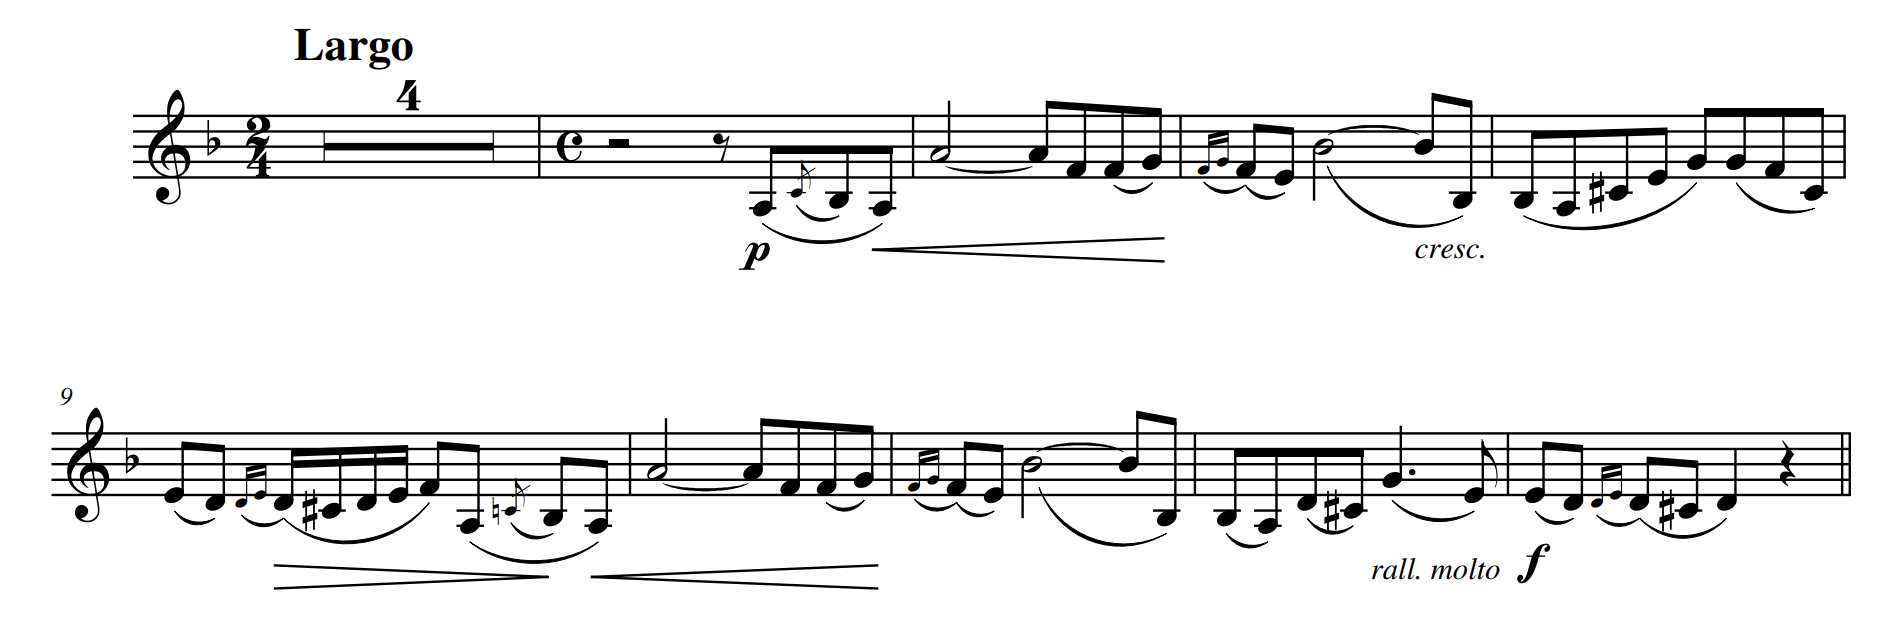
\includegraphics{img/czardas_partition.png}
\caption{Partition de la Largo de Csárdás (Vittorio Monti) pour violon}
\end{figure}

On voit bien un bémol à la clé \emph{(Fa majeur)}.

\hypertarget{tempo-et-rythme}{%
\subsection{Tempo et rythme}\label{tempo-et-rythme}}

le temps en musique se définit par le tempo et le rythme.

On définit d'abord \textbf{un temps} (en: \textbf{\emph{beat}}) l'unité
de temps en musique.

Le \textbf{tempo} du morceau est sa vitesse, il peut être décrit en
\textbf{BPM} (Beats per minute, fr: \emph{temps par minute}) ou bien par
un mot clé en italien: \emph{Largo, Andante, Allegro, Moderato, Lento,
Presto, etc} ce qui est moins précis mais bien compris par les
musiciens.

Le \textbf{rythme} du morceau est sa structure répétitive qui définit
une pulsation régulière.

La \textbf{mesure} est une structure \emph{rythmique} constitutées de
plusieurs \emph{temps} qui se répète périodiquement.

\begin{figure}
\centering
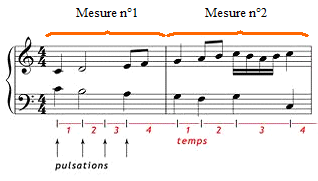
\includegraphics{img/rythme.png}
\caption{Rythme et tempo}
\end{figure}

La \textbf{métrique} (la division du temps) est le nombre de temps par
mesure \emph{et} la valeur d'un temps. Ce sont les 2 chiffres au début
d'un morceau, celui en bas indique le temps:

\begin{longtable}[]{@{}cccccc@{}}
\toprule
\textbf{Temps} & ronde & blanche & noire & croche &
double-croche\tabularnewline
\midrule
\endhead
\textbf{Nombre} & 1 & 2 & 4 & 8 & 16\tabularnewline
\bottomrule
\end{longtable}

Celui en haut indique le nombre de temps (beats) par mesure, par exemple
\(\frac{3}{4}\) est la métrique qui contient 3 noires par mesure. Les
unités les plus utilisées sont les noires et les croches, et rarement la
blanche.

\hypertarget{relation-entre-le-temps-et-tempo}{%
\subsection{Relation entre le temps et
tempo}\label{relation-entre-le-temps-et-tempo}}

Il se peut que la métrique soit changé dans un morceau. De plus, le
tempo n'est pas forcément constant. Même son évolution au cours du
morceau n'est pas toujours linéaire, on peut ralentir au milieu d'un
morceau jusqu'à l'arrêt total pour reprendre en plein vitesse d'un seul
coup.

On n'a donc aucune guarantie sur la régularité du tempo.

En revanche, afin de pouvoir tirer des résultats de notre analyse
précédantes on a dû prendre des cas particuliers suffisamment réguliers.
Par la suite, nous avons définit un \textbf{pseudo-PGCD} de durées de
notes, et nous avons divisés toutes les durées par ce nombre, et puis en
arrondissant le résultats nous avons obtenus des résultats qu'on a écrit
en format MIDI.

\hypertarget{ecriture-en-format-midi}{%
\subsection{Ecriture en format MIDI}\label{ecriture-en-format-midi}}

On reprend le morceau du piano afin d'obtenir une fonction constante par
morceau avec le temps en \emph{beats}, ce qu'on enregistra en format
MIDI grâce à la librarie python \texttt{midiutil}

\begin{Shaded}
\begin{Highlighting}[]
\ImportTok{from}\NormalTok{ muallef }\ImportTok{import}\NormalTok{ notes}
\NormalTok{time, pitch }\OperatorTok{=}\NormalTok{ notes.detect(fur_elise.signal, fur_elise.sampleRate)}
\NormalTok{plt.clf()}
\NormalTok{plot_step_function(time, pitch)}
\NormalTok{plt.show()}
\end{Highlighting}
\end{Shaded}

\includegraphics{index_files/figure-latex/unnamed-chunk-14-1.pdf}

\begin{Shaded}
\begin{Highlighting}[]
\NormalTok{notes.extract.extract_midi(time, pitch, }\StringTok{"fur_elise.midi"}\NormalTok{)}
\end{Highlighting}
\end{Shaded}

On compare la partition obtenue avec la partition originale:

\begin{figure}
\centering
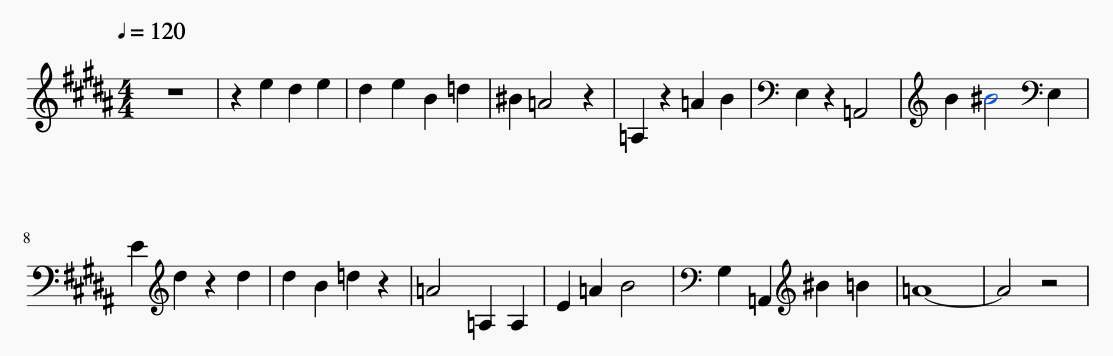
\includegraphics{img/fur_elise_midi.png}
\caption{Partition obtenue}
\end{figure}

\begin{figure}
\centering
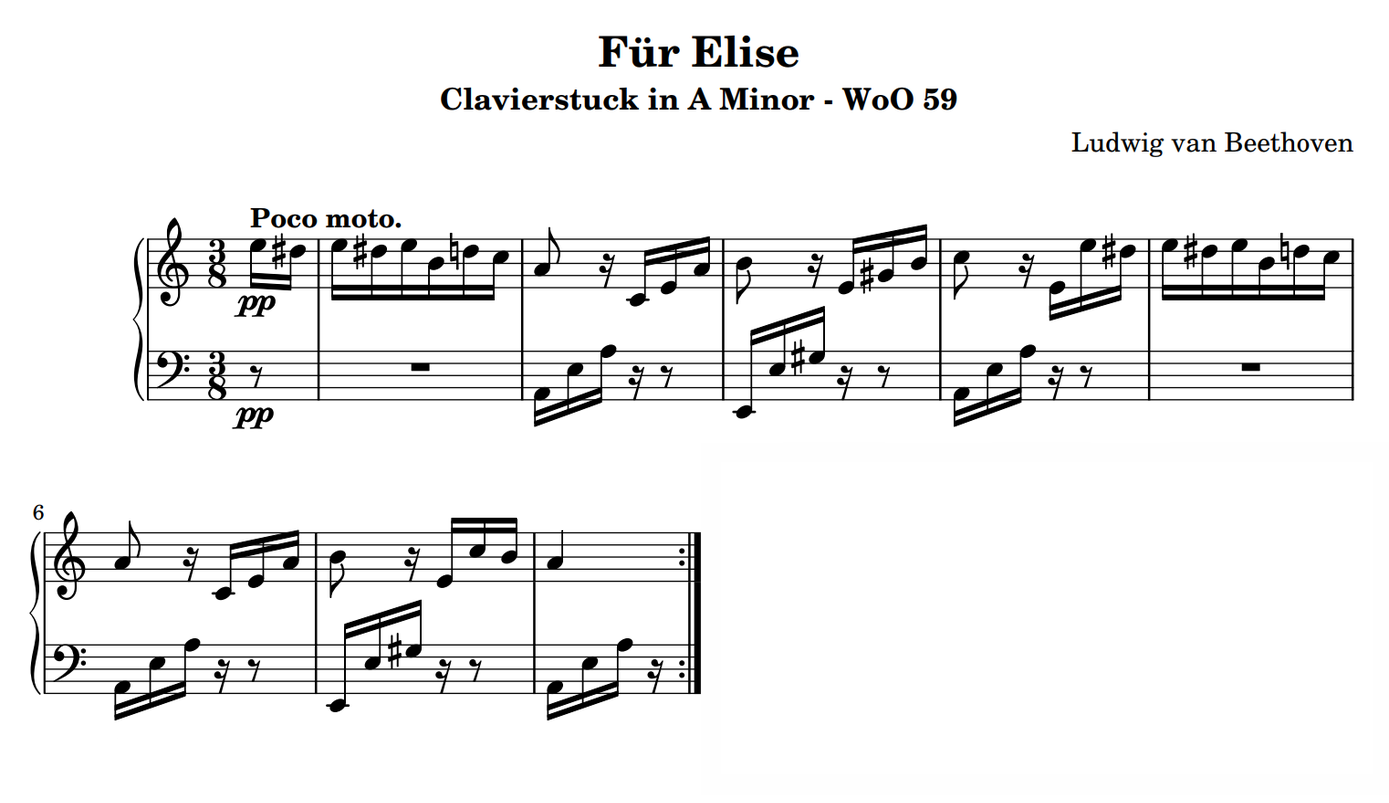
\includegraphics{img/fur_elise_partition.png}
\caption{Partition obtenue}
\end{figure}

On n'a pas obtenu les résultats qu'on espérait avoir, ceci pourra être
expliqué par 3 raisons:

\begin{itemize}
\tightlist
\item
  Notre implémentation ne traitent que les son monophones, mais ce
  morceau contient plusieurs notes simultanées différentes.
\item
  Le morceau est en La mineur (même armure que Do majeur), une gamme
  sans altérations. Or, dans les 2 lignes qu'on a traités nous avons
  croisé 3 dièses, d'où l'erreur dans le choix de la gamme.
\item
  Notre traitement du tempo est très élèmentaire, ici on a une métrique
  composée ce qui est un cas assez délicat pour tel programme.
\end{itemize}

En revanche, la ségmentation temporelle et la détéction de pitch sont
bien réussis.

\pagebreak

\hypertarget{conclusion}{%
\section{Conclusion}\label{conclusion}}

\hypertarget{resultats-1}{%
\subsection{Résultats}\label{resultats-1}}

Nous avons réussi à obtenir des résultats certainement intéressants,
mais nous n'avons pas pu tout implémenter car nous avons passé beaucoup
de temps à la recherche vu la nouveauté du sujet.

Nous aurions aimé pouvoir faire plus de tests avec des exemples variés.

\hypertarget{developpement-possible}{%
\subsection{Développement possible}\label{developpement-possible}}

Nous avons testé les librairies existantes:

\begin{itemize}
\tightlist
\item
  \url{aubio.org}
\item
  \url{essentia.upf.edu}
\item
  \url{librosa.github.io}
\end{itemize}

Les résultats sont assez satisfaisants. En revanche, ce domaine a du
fort potentiel de développement. Notamment le cas de musique pholyphone,
et dans la reconnaissance du rythme. D'après ma recherche, le plus
intéressant sera de faire intervenir de l'Intelligence Artificielle, en
particulier la technologie Long short-term Memory (LSTM). (Wikipedia
contributors 2018)

\hypertarget{apport-personnel}{%
\subsection{Apport personnel}\label{apport-personnel}}

Nous avons proposé ce projet par passion et motivation, ce qui nous a
poussé à faire de la recherche scientifique pour la première fois dans
notre vie académique.

Nous vous remercions sincèrement pour cette opportunité.

\pagebreak

\hypertarget{references}{%
\section*{Références}\label{references}}
\addcontentsline{toc}{section}{Références}

\hypertarget{refs}{}
\leavevmode\hypertarget{ref-phase}{}%
Bello, Juan, and Mark Sandler. 2003. ``Phase-Based Note Onset Detection
for Music Signals.''

\leavevmode\hypertarget{ref-yinfft}{}%
Brossier, Paul. 2007. ``Automatic Annotation of Musical Audio for
Interactive Applications.''

\leavevmode\hypertarget{ref-complex}{}%
Duxbury, Chris, Juan Bello, Mike Davies, and Mark Sandler. 2003.
``Complex Domain Onset Detection for Musical Signals.''

\leavevmode\hypertarget{ref-yin}{}%
Kawahara, Hideki, and Alain de Cheveigné. 2002. ``YIN, a Fundamental
Frequency Estimator for Speech and Music.''

\leavevmode\hypertarget{ref-hfc}{}%
Masri, Paul. 1996. ``Computer Modeling of Sound for Transformation and
Synthesis of Musical Signal.''

\leavevmode\hypertarget{ref-ismir}{}%
Rosão, Carlos, Ricardo Ribeiro, and David Martins de Matos. 2012.
``Influence of Peak Selection Methods on Onset Detection.''

\leavevmode\hypertarget{ref-lstm}{}%
Wikipedia contributors. 2018. ``Long Short-Term Memory --- Wikipedia,
the Free Encyclopedia.''
\url{https://en.wikipedia.org/w/index.php?title=Long_short-term_memory\&oldid=844880987}.

\leavevmode\hypertarget{ref-ougarit}{}%
Wikipédia. 2018. ``Chants Hourrites --- Wikipédia, L'encyclopédie
Libre.''
\url{http://fr.wikipedia.org/w/index.php?title=Chants_hourrites\&oldid=145548895}.


\end{document}
